% @Author: AnthonyKenny98
% @Date:   2020-02-23 14:27:21
% @Last Modified by:   AnthonyKenny98
% @Last Modified time: 2020-04-10 12:58:15

\subsection{Project Goals}
RISC-V was released 9 years ago. While it is starting to gain some traction in the commercial space, RISC-V has not yet been used to develop a motion planning specific processor. As such, the overall mission of this thesis is as follows:

\begin{center}
\bigskip\noindent\fbox{
    \parbox{0.8\textwidth}{
    \begin{center}
        \textbf{Mission} \\
        To present a proof-of-concept for extending and implementing RISC-V to develop motion planning specific processors.
    \end{center}
    }
} \\
\end{center}

\noindent To achieve this, the following objectives will need to be acheived:

\begin{center}
\bigskip\noindent\fbox{
    \parbox{0.9\textwidth}{
        \begin{center}        
        \textbf{Project Objectives} \\
        \end{center}
        \begin{enumerate}
            \item Determine the computational bottleneck of a commonly used motion planning algorithm.
            \item Implement a functional hardware module to replace the bottleneck function.
            \item Define a motion planning extension to the RISC-V ISA 
            \item Build a fully functional motion-planning processor that implements the extended RISC-V ISA
        \end{enumerate}
    }
} \\
\end{center}

\subsection{Project Structure}
    Chapter 2 details how \glsfirst{RRT}, a commonly used motion planning algorithm, is implemented and analysed. From this analysis, it is determined that the computational bottleneck is edge collision detection. Chapter 3 outlines a process for implementing this bottleneck function in a hardware module, achieving a $5 \times$ speedup. Chapter 4 defines the RISC-V  motion planning extension and describes the build of a RISC-V processor that implements this extension and the Honeybee unit.

    \newpage
    \subsubsection{Computer Implementation Hierarchy}
        To briefly frame the space in which this thesis operates, consider the hierarchy of computer implementation, demonstrated in Figure \ref{fig:computerHierarchy}. \textbf{User level applications}, such as Microsoft Word, Google Chrome, and Apple's iTunes, sit at the top of the hierarchy. These applications are implemented in \textbf{High/Mid Level Languages}, such as C/, C++, Python, Java, etc. 
        This software is eventually executed on a \textbf{Processor}, otherwise known as a \gls{CPU}. A processor does not understand Python, or any other programming language for that matter. The only thing it can understand is binary values (a one or a zero). Every computer program gets translated into ones and zeros (called machine code) for execution on a processor. But how are languages like C translated into machine code? The layer between programming languages and the processor is the \textbf{Instruction Set Arcitecture (ISA)}. Chapter 4 goes into detail about \gls{ISA}s and how they work. For now, if unfamiliar with the topic, it is sufficient to think of an \gls{ISA} as a translator between programming languages and machine code. This thesis operates across the lower three levels of this hierarchy.
        
        % @Author: AnthonyKenny98
% @Date:   2020-02-29 23:52:30
% @Last Modified by:   AnthonyKenny98
% @Last Modified time: 2020-04-10 12:37:43
\begin{figure}[H]
\begin{center}
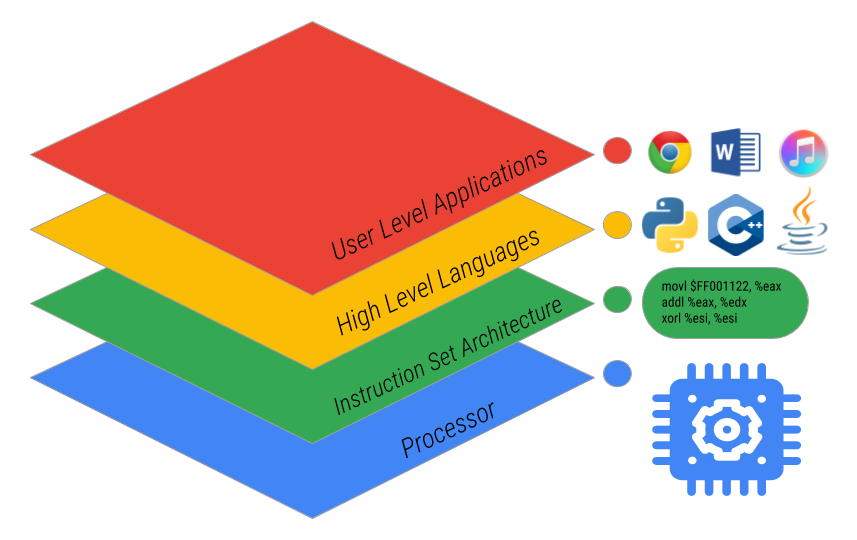
\includegraphics[width=\linewidth]{chapters/chapter1/img/computerHierarchy.png}
\mycaption{Simple Visualization of Computer Implementation Hierarchy}{}
\label{fig:computerHierarchy}
\end{center}
\end{figure}


    \subsubsection{System Overview}
        Figure \ref{fig:systemDiagram} shows a high level overview of the system this thesis proposes.
        % @Author: AnthonyKenny98
% @Date:   2020-03-01 11:14:04
% @Last Modified by:   AnthonyKenny98
% @Last Modified time: 2020-03-01 11:45:10
\begin{figure}[H]
\begin{center}
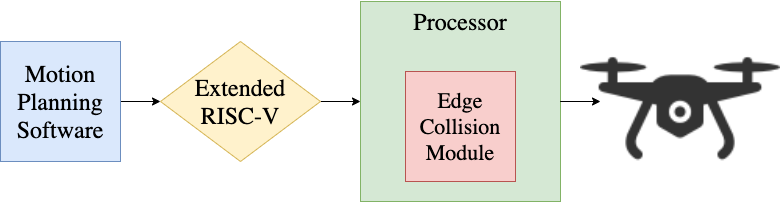
\includegraphics[width=\linewidth]{chapters/chapter1/img/systemDiagram.png}
\caption{System Diagram of Overall Project}
\label{fig:systemDiagram}
\end{center}
\end{figure}
        The \textbf{Extended RISC-V \gls{ISA}} is made up of the \gls{RV32I} Base Instruction Set and a \ifdraft{\color{red}\textbf{currently unnamed}\color{black}} non-standard extension that this thesis will define.
        The \textbf{PhilosophyV Processor} is a RISC-V chip built in \gls{HDL} for this thesis. It implements both the \gls{RV32I} instruction set and the non-standard extension.
        The PhilosphyV Core includes, along with a baseline 5-stage processor implementation, the \textbf{HoneyBee} collision detection unit.
        A \textbf{C Implementation of RRT} is loaded into the instruction memory of the PhilosophyV processor. This processor, synthesized on an \textbf{\gls{FPGA}}, is used as the main processor, co-processor, or accelerator on an \textbf{Autonomous \gls{UAV}}. Table \ref{table:componentList} outlines the components of this system and their descriptions.
        % @Author: AnthonyKenny98
% @Date:   2020-03-01 12:32:47
% @Last Modified by:   AnthonyKenny98
% @Last Modified time: 2020-03-01 13:59:51
\begin{table}[H]
\begin{center}
\begin{tabular}{|p{.2\linewidth}|p{.2\linewidth}|p{.5\linewidth}|}
    \hline
    \textbf{Component}          & \textbf{Source}   & \textbf{Description} \\
    \hline
    \multicolumn{3}{|c|}{RISC-V Instruction Set} \\
    \hline
    \ac{RV32I}              & Berkeley & 40 Instructions defined such that \ac{RV32I} is sufficient to form a compiler target and suport modern operating systems \cite{Waterman2019}. \\
    \hline
    Extension        & \textit{New} & This is the custom extension defined by this thesis targeting motion planning instructions. It is outlined in Chapter \ref{chap:RiscvProcessor}. \\
    \hline
    \multicolumn{3}{|c|}{C-Implementation of RRT} \\
    \hline
    RRT        & \textit{New} & Due to lack of available implementations of \ac{RRT} suitable for the purposes of this thesis, \ac{RRT} was implemented from the ground up in C. This is detailed in Chapter \ref{chap:MotionPlanningInSoftware} \\
    \hline
    \multicolumn{3}{|c|}{FPGA Synthesized Chip} \\
    \hline
    Zynq-7000        & Xilinx & The Zynq-7000 family of \ac{SoC}s are a low cost FPGA and \ac{ARM} combined unit. \\
    \hline
    PhilosophyV     & \textit{New} & The processor built for this thesis to demonstrate how the RISC-V extension and hardware unit work together. This is detailed in Chapter \ref{chap:RiscvProcessor} \\
    \hline
    HoneyBee        & \textit{New} & The functional unit designed specifically for faster execution of edge collision detection computations. Outlined in Chapter \ref{chap:MotionPlanningInHardware} \\
    \hline
\end{tabular}
\caption{List of System Components and their Descriptions}
\label{table:componentList}
\end{center}
\end{table}

    \todo[inline]{Update Above Table}

\subsection{Project Specifications}

    \todo[inline, caption={Project Specifications}]{This can just be the stuff from the start. Objective and 4 goals}

\subsection{Project Structure}
\label{subsection:project_structure}
    This report is structured to follow the timeline of this project, and is outlined below:
    \begin{enumerate}
        \item A benchmark motion planning algorithm, \gls{RRT}, was selected and implemented in software. Once implemented, a variety of performance analysis methods were used to profile the computational hotspots of the algorithm. It was found that edge collision detection was the critical function limiting execution time. This process is detailed in Chapter 2.
        \item With edge collision detection having been identified as the critical function, the process of designing specialised hardware to execute this function began. The technical specifications, performance specifications, designs, build phases, measurement and analysis of this hardware unit is presented in Chapter 3.
        \item With the aforementioned functional unit's performance verified in simulation, the next step was to implement this in a processor. First, a baseline processor was designed and built for this project to implement a base RISC-V instruction set. The performance of \gls{RRT} is again profiled on this baseline processor (as up until this point, it was profiled on x86 architecture). A non-standard extension to the RISC-V \gls{ISA} was then defined and support for this was implemented in the processor. Comparative performance analysis was then conducted. This process is described in detail in Chapter 4.
        \item Chapter 5 is a discussion of results and future work.
    \end{enumerate}

\subsubsection{extending riscv}
 RISC-V is designed cleverly in a modular way, with a set of base instruction sets and a set of standard extensions. As a result, processors can be designed to only implement the instruction groups it requires, saving time, space and power on instructions that won't be used. In addition, another goal of RISC-V is to provide a basis for more specialized instruction-set extensions or more customized accelerators. This is described in the most recent \textit{RISC-V Instruction Set Manual} \cite{Waterman2019}. This is a powerful feature, as it does not break any software compatability, but allows for designers to easily follow the steps outlined in Figure \ref{fig:extendingRISCV}. From a \gls{hardware acceleration} point of view, this is particularly useful as it allows the designer to directly invoke whatever functional unit or accelerator they implement from assembly code.
    % @Author: AnthonyKenny98
% @Date:   2020-03-01 10:28:34
% @Last Modified by:   AnthonyKenny98
% @Last Modified time: 2020-03-01 10:32:45
\begin{figure}[H]
\begin{center}
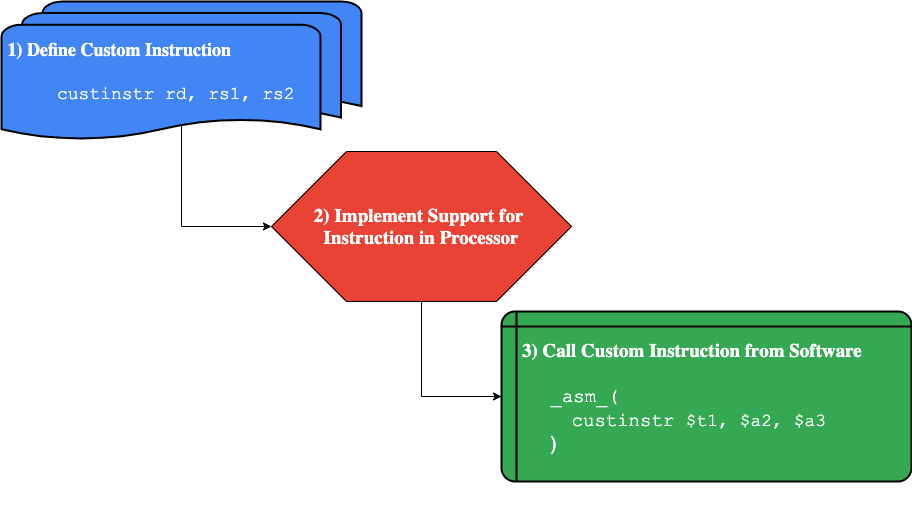
\includegraphics[width=0.9\linewidth]{chapters/chapter1/img/extendingRISCV.png}
\caption{Typical Process of Adding Non-Standard Extension to RISC-V ISA}
\label{fig:extendingRISCV}
\end{center}
\end{figure}

\todo[inline,caption={Summary of Results}]{Do I need a summary of results section in the introduction? }